\documentclass[a4paper]{article}
\usepackage{pgf,tikz,pgfplots}
\usetikzlibrary{arrows,decorations.markings}
\pgfplotsset{compat=1.15}
\usepackage{mathrsfs}
\usetikzlibrary{arrows}
%% Language and font encodings
\usepackage[english]{babel}
\usepackage[utf8x]{inputenc}
\usepackage[T1]{fontenc}
\usepackage{float}
%% Sets page size and margins
\usepackage[a4paper,top=3cm,bottom=2cm,left=3cm,right=3cm,marginparwidth=1.75cm]{geometry}
\usepackage{fancyhdr}
\pagestyle{fancy}
%% Useful packages

\usepackage{amsmath}
\usepackage{amsthm}
\usepackage{enumitem}
\usepackage{eqnarray}
\usepackage{float}
\usepackage{esint}
\usepackage{wrapfig}
\usepackage{gensymb}
\usepackage{lipsum}
\usepackage{amssymb}
\usepackage{array}
\usepackage{tikz}
\usepackage[colorlinks=true, allcolors=blue]{hyperref}
\usepackage{graphicx}
\usepackage{amsmath}
\usepackage{amssymb}
\usepackage{graphicx}
\usepackage[colorlinks=true, allcolors=blue]{hyperref}
\usepackage{mathtools}
\DeclareMathOperator{\Proj}{Proj}
\DeclareMathOperator{\lcm}{lcm}
\DeclareMathOperator{\cosec}{cosec}
\DeclareMathOperator{\sgn}{sgn}
\DeclareMathOperator{\Span}{span}
\DeclareMathOperator{\nullity}{nullity}
\DeclarePairedDelimiter\floor{\lfloor}{\rfloor}
\DeclareMathOperator{\Res}{Res}
\DeclareMathOperator{\rank}{rank}
\DeclareMathOperator{\Ker}{Ker}
\DeclareMathOperator{\R}{R}
\DeclareMathOperator{\Tr}{Tr}
\DeclareMathOperator{\diag}{diag}
\DeclareMathOperator{\Log}{Log}
\DeclareMathOperator{\sech}{sech}
\DeclareMathOperator{\Var}{Var}
\newtheorem{ans}{Answer}[subsection]

\definecolor{darkblue}{RGB}{	0, 0, 139}
\newtheoremstyle{new}% <name>
{2pt}% <Space above>
{2pt}% <Space below>
{\color{darkblue}}% Body font
{}% <Indent amount>
{\bfseries\color{black}}% Theorem head font
{:}% <Punctuation after theorem head>
{.5em}% <Space after theorem headi>
{}% <Theorem head spec (can be left empty, meaning `normal')>
\theoremstyle{new}
\newtheorem{qns}{Problem}[section]
\setlength{\parindent}{0cm}
\title{\textbf{Part II REL Problem Sheet Solutions}}
\author{Tai Yingzhe, Tommy (ytt26)}
\date{}
\setlength{\parindent}{0cm}
\begin{document}
\maketitle
\tableofcontents
\newpage
\section{Problem Sheet 1}
\subsection*{Special Relativity}
\begin{qns}[Spacetime interval]\leavevmode
\begin{enumerate}[label=(\alph*)]
\item Show that if two events are separated by a timelike interval, then there is a frame in which they occur at the same spatial location.
\item Similarly, if two events are separated by a spacelike interval, show there is a frame in which they are simultaneous.
\end{enumerate}
\end{qns}
\begin{ans}\leavevmode
\begin{enumerate}[label=(\alph*)]
\item Without loss of generality, align axes of $S$ such that $\Delta y=\Delta z=0$. Perform standard Lorentz boost to another frame $S'$:
$$\Delta y'=\Delta z'=0,\quad\Delta x'=\gamma(\Delta x-\frac{v}{c}\Delta t)$$
To ensure they occur at the same spatial location in frame $S'$:
$$\Delta x'=0\implies\frac{v}{c}=\frac{\Delta x}{c\Delta t}\implies|\Delta x|<c|\Delta t|$$
The spacetime interval is
$$\Delta s^2=(c\Delta t)^2-(\Delta x)^2-(\Delta y)^2-(\Delta z)^2=(c\Delta t)^2-(\Delta x)^2-0>0$$
and hence the events are time-like separated.
\item Again without loss of generality, $\Delta y=\Delta z=0$. Perform a standard Lorentz boost, i.e. $c\Delta t'=\gamma(c\Delta t-\beta\Delta x)$. For two events to be simultaneous in frame $S'$, $\Delta t'=0$, we have $$\beta=\frac{c\Delta t}{\Delta x}\implies\frac{\Delta t}{\Delta x}=\frac{\beta}{c}<1\implies c\Delta t<\Delta x$$
The spacetime interval is
$$\Delta s^2=(c\Delta t)^2-(\Delta x)^2-(\Delta y)^2-(\Delta z)^2=(c\Delta t)^2-(\Delta x)^2-0<0$$
and hence the events are space-like separated.
\end{enumerate}
\end{ans}
\begin{qns}[Spacetime interval]\leavevmode
\begin{enumerate}[label=(\alph*)]
\item Show that if an event A precedes an event B in some frame S at the same spatial location, then the event A precedes event B in all frames. 
\item Two general events A and B are separated in S by a spatial distance $\Delta r$. If event A causes event B, determine an inequality for the time difference between the events, $\Delta t=t_B-t_A$. Hence show that the events are causally related in all frames.
\end{enumerate}
\end{qns}
\begin{ans}\leavevmode
\begin{enumerate}[label=(\alph*)]
\item In frame $S$, if two events occur at the same spatial location $\Delta\mathbf{r}=\boldsymbol{0}$, then $\Delta t=t_B-t_A>0$, i.e. event A precedes event B. Under standard Lorentz boost,
$$c\Delta t'=\gamma(c\Delta t)>0$$
Hence $\Delta t'>0$ $\forall\gamma$, i.e. for all frames related to $S$ by a Lorentz boost.
\item If A causes B, time is needed for a signal to propagate between them, i.e. $c\Delta t>\Delta r\implies\Delta s^2=(c\Delta t)^2-(\Delta\mathbf{r})^2>0$. By invariance of the spacetime interval, we must have $|c\Delta t'|>|\Delta\mathbf{r'}|$ in any frame. Choose axes in $S$ and $S'$ so in standard configuration,
$$\Delta x\leq\Delta r,~c\Delta t>\Delta r\implies c\Delta t'=\gamma(c\Delta t-\beta\Delta x)>0\implies c\Delta t'>|\Delta\mathbf{r}|$$
Hence, the two events are causally related in all frames.
\end{enumerate}
\end{ans}
\newpage
\begin{qns}[Spacetime diagram]\leavevmode
\begin{enumerate}[label=(\alph*)]
\item On a spacetime diagram with the $x$ and $ct$ axes of an inertial frame $S$ horizontal and vertical, respectively, construct the lines of constant $x'$ and $ct'$, where these coordinates refer to the frame $S'$ in standard configuration with $S$ (i.e., where $S'$ moves at a speed $v$ along the positive $x$-direction and the two frames coincide at $t = t' = 0$). Show that the angle between the $x$- and $x'$- axes is the same as that between the $ct$- and $ct'-$ axes and has the value $\tan^{-1}(v/c)$.
\item Sketch on your diagram the loci of events separated from the spacetime origin $x = ct = 0$ by a constant invariant interval $\Delta s^2=c^2t^2-x^2$ for positive (timelike) and negative (spacelike) values of $\Delta S^2$. How can these curves be used to calibrate lengths along the axes of the $S$ and $S'$ frames?
\item Use your diagram to illustrate graphically why a rod at rest in $S'$ is \textit{contracted} as measured in $S$, and the time on a clock at rest in $S'$ is \textit{dilated} as observed in $S$.
\end{enumerate}
\end{qns}
\begin{ans}\leavevmode
\begin{enumerate}[label=(\alph*)]
\item The lines of constant $t'$ and $x'$ have equations $ct'=\gamma(ct-\beta x)=\text{const.}$ and $x'=\gamma(x-\beta ct)=\text{const.}$. The angle between the $x$ and $x'$-axes is
$$\tan^{-1}(x'/ct)=\tan^{-1}(\beta)$$
The angle between the $ct'$ and $ct$-axes is
$$\tan^{-1}(x/ct)=\tan^{-1}(\beta)$$
where $\beta=v/c$.
\item The spacetime interval is $\Delta s^2=c^2t^2-x^2$ and are represented by hyperbolae. On the spacetime diagram below, we have $\Delta s^2<0$ and $\Delta s^2>0$ to be represented by the red and blue curves respectively. The diagonal asymptotes are the worldlines of photons starting at the common spacetime origin, travelling at $\pm c$.
\begin{center}
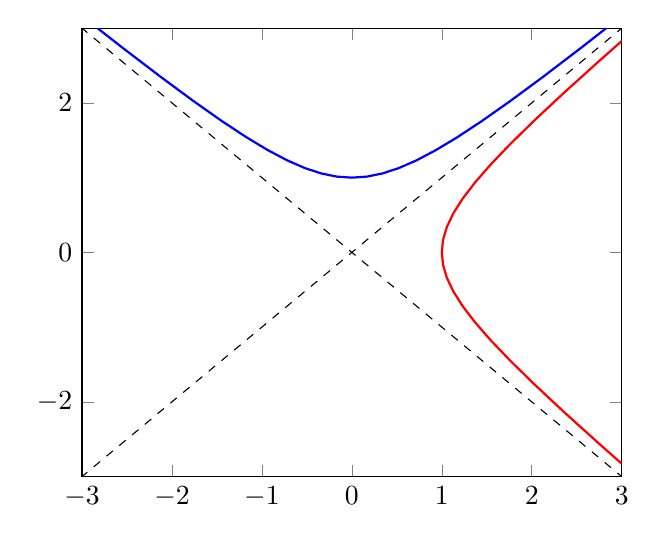
\begin{tikzpicture}
    \begin{axis}[
            xmin=-3,xmax=3,
        ymin=-3,ymax=3]
        \addplot [red,thick,domain=-2:2] ({cosh(x)}, {sinh(x)});
        \addplot [blue,thick,domain=-2:2] ({sinh(x)}, {cosh(x)});
        \addplot[black,dashed] expression {x};
        \addplot[black,dashed] expression {-x};
    \end{axis}
\end{tikzpicture}
\end{center}
Consider $\Delta s^2=-1$, then this hyperbola intersects the $x$ and $x'$-axes at $x=1$ and $x'=1$ respectively.
\item The fact that the spacetime interval hyperbolic curves can be used to calibrate lengths along the axes of the $S$ and $S'$ frames, we can demonstrate length contraction and time dilation. 
\begin{itemize}
    \item Time dilation: Suppose we have a clock with worldline $x'=0$ $\forall t'$ which measures a period $ct'=cT_0$. The spacetime interval curve $\Delta s^2=c^2T_0^2$ connects points on the $ct'$- and $ct$-axes with length $cT_0$. In frame $S$ however, the observer measures the event with period $ct=c\Delta t$ instead, which graphically we have $c\Delta t>cT_0$, i.e. time dilated in $S$.
    \item Length contraction: Suppose we have a rod of length $\ell_0$ at rest in frame $S'$. Again, the hyperbola $\Delta s^2=-\ell_0^2$ connects points on the $x'$- and $x$-axes with length $\ell_0$. To measure the length of the rod $\Delta x$ in $S$, we need to mark out the positions of both ends simultaneously. We can see graphically that $\ell_0>\Delta x$, i.e. length contraction in $S$.
\end{itemize}
\end{enumerate}
\end{ans}
\newpage
\begin{qns}[Lorentz boost]
An inertial frame $S'$ is related to the frame $S$ by a boost of $\vec{v}$ whose components in $S$ are $(v_x, v_y, v_z)$. Show that the coordinates $(ct', x', y', z')$ and $(ct, x, y, z)$ of an event are related by
$$\begin{pmatrix}ct'\\x'\\y'\\z'\\\end{pmatrix}=\begin{pmatrix}\gamma&-\gamma\beta_x&-\gamma\beta_y&-\gamma\beta_z\\-\gamma\beta_x&1+\alpha\beta_x^2&\alpha\beta_x\beta_y&\alpha\beta_x\beta_z\\-\gamma\beta_y&\alpha\beta_y\beta_x&1+\alpha\beta_y^2&\alpha\beta_y\beta_z\\-\gamma\beta_z&\alpha\beta_z\beta_x&\alpha\beta_z\beta_y&1+\alpha\beta_z^2\\\end{pmatrix}\begin{pmatrix}ct\\x\\y\\z\\\end{pmatrix}$$
where $\vec{\beta}=\vec{v}/c$, $\gamma=(1-|\vec{\beta}|^2)^{-1/2}$ and $\alpha=(\gamma-1)/|\vec{\beta}|^2$. (Hint: resolve the 3-vector position with components $(x, y, z)$ into parallel and perpendicular parts with respect to $\vec{\beta}$, and similarly in the $S'$ frame.)
\end{qns}
\begin{ans}
Resolve $\mathbf{r}=(x,y,z)$ into parallel and perpendicular parts with respect to $\vec{\beta}$:
$$\mathbf{r}=(\mathbf{r}\cdot\hat{\vec{\beta}})\hat{\vec{\beta}}+[\mathbf{r}-(\mathbf{r}\cdot\hat{\vec{\beta}})\hat{\vec{\beta}}]:=r_\parallel\hat{\vec{\beta}}+\mathbf{r_{\perp}}$$
and similarly for $\mathbf{r'}=(x',y',z')$. For a standard Lorentz Boost, the components perpendicular to $\hat{\vec{\beta}}$ are unchanged and that parallel transform as usual, i.e.
$$r_\parallel'=\gamma(r_\parallel-\beta ct),\quad\mathbf{r_\perp'}=\mathbf{r_{\perp}},\quad ct'=\gamma(ct-\beta r_\parallel)$$
Hence, we have
$$\mathbf{r'}=r_\parallel'\hat{\vec{\beta}}+\mathbf{r}-r_\parallel\hat{\vec{\beta}}=-\gamma\beta ct\hat{\vec{\beta}}+\bigg[\text{Id}+(\gamma-1)
\begin{pmatrix}\hat{\beta}_x^2&\hat{\beta}_x\hat{\beta}_y&\hat{\beta}_x\hat{\beta}_z\\
\hat{\beta}_y\hat{\beta}_x&\hat{\beta}_y^2&\hat{\beta}_y\hat{\beta}_z\\
\hat{\beta}_z\hat{\beta}_x&\hat{\beta}_z\hat{\beta}_y&\hat{\beta}_z^2\\\end{pmatrix}\bigg]\mathbf{r}$$
but $\gamma-1=\alpha|\vec{\beta}|^2$, and so
$$\mathbf{r'}=-\gamma\beta \hat{\vec{\beta}}ct+\begin{pmatrix}1+\alpha\beta_x^2&\alpha\beta_x\beta_y&\alpha\beta_x\beta_z\\\alpha\beta_y\beta_x&1+\alpha\beta_y^2&\alpha\beta_y\beta_z\\\alpha\beta_z\beta_x&\alpha\beta_z\beta_y&1+\alpha\beta_z^2\\\end{pmatrix}\mathbf{r}$$
Together with
$$ct'=\gamma ct-\gamma\beta(x\beta_x+y\beta_y+z\beta_z)$$
We have our desired answer.
\end{ans}
\begin{qns}[Velocity composition]
In a given inertial frame, two particles are shot out simultaneously from a given
point, with equal speeds v in orthogonal directions. What is the speed of each particle
relative to the other?
\end{qns}
\begin{ans}
Let particle A and B have velocities $v(0,1,0)$ and $v(1,0,0)$ respectively. In the frame of particle B (Lorentz boost by $v(1,0,0)$), particle B observes particle A to have $u_x=0$, $u_y=v$, $u_z=0$ and so by usual velocity transformation,
$$u_x'=-v,\quad u_y'=v/\gamma_v,u_z'=0$$
The relative speed is then $v(1+\gamma_v^{-2})^{1/2}=v(2-(v/c)^2)^{-1/2}$.
\end{ans}
\newpage
\begin{qns}[Velocity composition]\leavevmode
\begin{enumerate}[label=(\alph*)]
\item Frame $S'$ moves with speed $v$ relative to frame $S$ in standard configuration. A rod at rest in frame $S'$ makes an angle $\theta'$ with respect to the forward direction of motion. What is the angle $\theta$ measured in S?
\item If a bullet is fired in $S'$ at speed $u'$ at an angle $\theta'$ with respect to the forward direction of motion, what is the angle $\theta$ measured in $S$? What if the bullet is a photon?
\end{enumerate}
\end{qns}
\begin{ans}\leavevmode
\begin{enumerate}[label=(\alph*)]
\item Let the two ends of the rod (with proper length $\ell_0$) be A and B where A is at the origin. The worldline of A has coordinates $(ct',0,0,0)$ in frame $S'$. The wordline of B has coordinates $(ct',\ell_0\cos\theta',\ell_0\sin\theta',0)$. Inverse Lorentz transform back to frame $S$, the coordinates for A and B are respectively
$$\begin{pmatrix}\gamma ct'\\\gamma\beta ct'\\0\\0\\\end{pmatrix}=\begin{pmatrix}ct\\\beta ct\\0\\0\\\end{pmatrix},\quad\begin{pmatrix}\gamma ct'+\gamma\beta\ell_0\cos\theta'\\\gamma\ell_0\cos\theta'+\gamma\beta ct'\\\ell_0\sin\theta'\\0\\\end{pmatrix}=\begin{pmatrix}ct\\\gamma\ell_0\cos\theta'+\beta(ct-\gamma\beta\ell_0\cos\theta)=\ell_0\gamma^{-1}\cos\theta'+vt\\\ell_0\sin\theta'\\0\\\end{pmatrix}$$
The back and the front both moves at speed $v$, as expected. Hence, we must have
$$\tan\theta=\frac{\ell_0\sin\theta'}{\ell_0\cos\theta'/\gamma}=\gamma\tan\theta'$$
\item Inverse transform the velocity components for $u'$:
$$u_x=\frac{u'\cos\theta'+v}{1+(u'v/c^2)\cos\theta'},\quad ,u_y=\frac{u'\sin\theta'}{\gamma_v(1+(u'v/c^2)\cos\theta')},\quad u_z=0$$
The angle $\theta$ in $S$ satisfies
$$\tan\theta=\frac{u'\sin\theta'}{\gamma_v(u'\cos\theta'+v)}$$
If the object was a photon, then $u=c$ and we recover the light aberration relation $\tan\theta=\frac{\sin\theta'}{\gamma_v(\cos\theta'+\beta)}$.
\end{enumerate}
\end{ans}
\begin{qns}
Frame $S'$ moves with speed $v$ relative to frame $S$ in standard configuration. Neutral $\pi$-mesons at rest in $S'$ decay into two photons that are emitted isotropically. Show that the angular distribution of photons in $S$ is
$$P(\theta)d\theta=\frac{\sin\theta d\theta}{2\gamma^2(1-\beta\cos\theta)^2}$$
\end{qns}
\begin{ans}
From Q6, we have 
$$\cos\theta'=\frac{\cos\theta-\beta}{1-\beta\cos\theta}\implies\frac{d\cos\theta'}{d\cos\theta}=\frac{1-\beta\cos\theta-(\cos\theta-\beta)(-\beta)}{(1-\beta\cos\theta)^2}=\frac{1}{\gamma^2(1-\beta\cos\theta)^2}$$
Photons are emitted isotropically in a solid angle $2\pi~ d(\cos\theta')$ in $S'$ are emitted in a solid angle $2\pi~d(\cos\theta)$ in $S$. The number of photons emitted in either frame is the same:
$$P(\theta)d\theta=P(\theta')d\theta'=\frac{1}{4\pi}2\pi~d\cos\theta'\implies P(\theta)d\theta=\frac{1}{2}\frac{d(\cos\theta')}{d(\cos\theta)}\sin\theta d\theta=\frac{\sin\theta d\theta}{2\gamma^2(1-\beta\cos\theta)^2}$$
i.e. the photons are strongly `breamed' in the $x$-direction due to aberration.
\end{ans}
\newpage
\begin{qns}[Acceleration]\leavevmode
\begin{enumerate}[label=(\alph*)]
\item A spaceship travels in a straight line at a variable speed $u(t)$ in some inertial frame $S$. An observer on the spaceship measures his acceleration to be $f(\tau)$, where $\tau$ is his proper time. If at $\tau=0$ the spaceship has a speed $u_0$ in $S$ show that
$$\frac{u(\tau)-u_0}{1-u(\tau)u_0/c^2}=c\tanh\psi(\tau)$$
where $c\psi(\tau)=\int_0^\tau f(\tau')d\tau'$. Show that the speed of the spaceship can never reach $c$.
\item If the spaceship left base at time $t=\tau=0$ and travelled forever in a straight line with constant acceleration $g$ (for comfort), how long by the spaceship clock does it take to reach a star 10 light years from the base?
\end{enumerate}
\end{qns}
\begin{ans}\leavevmode
\begin{enumerate}[label=(\alph*)]
\item $f(\tau)$ is the acceleration in the instantaneous rest frame (IRF). At proper time $\tau$, the speed is $u$ and increases by $f(\tau)d\tau$ in the IRF. In $S$, the speed increases by $du$. By velocity addition,
$$u+du=\frac{fd\tau+u}{1+(u/c^2)fd\tau}=u\bigg(1-\frac{u}{c^2}fd\tau\bigg)+fd\tau+\dots=u+\frac{fd\tau}{\gamma_u^2}+\dots\implies\frac{du}{d\tau}=\frac{f}{\gamma_u^2}$$
Let $u/c=\tanh\theta(\tau)$, then
$$\frac{du}{d\tau}=\frac{c}{\cosh^2\theta}\frac{d\theta}{d\tau}\implies\frac{d\theta(\tau)}{d\tau}=\frac{f(\tau)}{c}$$
since $\gamma_u=\cosh\theta$ (definition of rapidity). We then have
$$c\theta(\tau)=\int_0^\tau f(\tau')d\tau'+c\tanh^{-1}(u_0/c)$$
where the integration constant occur since $u=u_0$ at $\tau=0$. Evaluate $\tanh\psi(\tau)$:
$$\tanh\psi=\tanh(\theta-\tanh^{-1}(u_0/c))=\frac{\tanh\theta-u_0/c}{1-(u_0/c)\tanh\theta}=\frac{1}{c}\frac{u-u_0}{1-uu_0/c^2}$$
Upon rearranging, we have
$$\frac{u}{c}=\frac{(u_0/c)+\tanh\psi}{1+(u_0/c)\tanh\psi}$$
For $0\leq\psi<\infty$, the RHS increases monotonically from $u_0/c$ to 1, i.e. $u(\tau)$ approaches but never exceeds $c$.
\item By definition of proper time,
$$c^2d\tau^2=c^2dt^2-dx^2=c^2dt^2(1-u^2/c^2)$$
We have $d\tau/dt=1/\gamma_u=1/\cosh\psi$, so since
$$u=\frac{dx}{d\tau}\frac{d\tau}{dt}=c\tanh\psi\implies\frac{dx}{d\tau}=c\sinh\psi$$
But $\psi(\tau)=(g/c)\int_0^\tau d\tau=g\tau/c$, so
$$x=\frac{c^2}{g}[\cosh(g\tau/c)-1]$$
where the integration constant is obtained from $x(\tau=0)=0$. We have $x=10$ light years and so $xg/c^2=\frac{(365.25)(24)(3600)(10)(9.81)}{3\times10^8}=10.32$ and hence $g\tau/c=\cosh^{-1}(10.32+1)=3.118$. Hence,
$$\tau=\frac{3.118}{9.81}\frac{3\times10^8}{24(3600)(365.25)}=3.02\text{ years}$$
\end{enumerate}
\end{ans}
\newpage
\subsection*{Manifolds and Coordinates}
\begin{qns}
In 3D Euclidean space, coordinates $x'^a$ are related to Cartesian coordinates $x^a$ by
$$x^1=x'^1+x'^2,\quad  x^2=x'^1-x'^2,\quad x^3=2x'^1x'^2+x'^3$$
Describe the coordinate surfaces in the primed system. Obtain the metric functions $g_{ab}'$ in the primed system and hence show that these coordinates are not orthogonal. Calculate the volume element $dV$ in the primed coordinate system.
\end{qns}
\begin{ans}
To describe the surfaces associated to the primed coordinates, we rearrange to get
$$x'^1=0.5(x^1+x^2),\quad x'^2=0.5(x^1-x^2),\quad x'^3=x^3-0.5((x^1)^2-(x^2)^2)$$
$x'^1=\text{const.}$ and $x'^2=\text{const.}$ are diagonal planes in the $x$-space, while $x'^3=\text{const.}$ are hyperbolic paraboloids with principal axes along $x^1$ and $x^2$ directions. The spacetime invariant is
\begin{align}
    ds^2&=(dx^1)^2+(dx^2)^2+(dx^3)^2\nonumber\\&=(dx'^1+dx'^2)^2+(dx'^1-dx'^2)^2+(2x'^1dx'^2+2dx'^2dx'^1+dx'^3)^2\nonumber\\&=2(dx'^1)^2+2(dx'^2)^2+4(x'^1)^2(dx'^2)^2+4(x'^2)^2(dx'^1)^2+(dx'^3)^2\nonumber\\&~~ +8x'^1x'^2~dx'^1~dx'^2+4x'^1~dx'^2+dx'^3+4x'^2~dx'^1~dx'^3\nonumber\\&=2(1+2(x'^2)^2)(dx'^1)^2+2(1+2(x'^1)^2)(dx'^2)^2+x'^1x'^2~dx'^1~dx'^2+4x'^1~dx'^2~dx'^3+4x'^2~dx'^1~dx'^3+(dx^3)^2\nonumber
\end{align}
with the metric tensor as
$$g'_{ab}=\begin{pmatrix}2(1+2(x'^2)^2)&4x'^1x'^2&2x'^2\\4x'^1x'^2&2(1+2(x'^1)^2)&2x'^1\\2x'^2&2x'^1&1\\\end{pmatrix}$$
Since the metric tensor is not diagonal, it is not an orthogonal coordinate system. The determinant and hence volume element is 
\begin{align}
    &\det g\nonumber\\&=2(1+2(x'^2)^2)[2(1+2(x'^1)^2-4(x'^1)^2]-4(x'^1)(x'^2)[4x'^1~x'^2-4x'^1~x'^2]+2x'^2[8(x'^1)^2(x'^2)-4(x'^2)(1+2(x'^1)^2)]\nonumber\\&=4\implies dV=\sqrt{\det g}dx'^1~dx'^2~dx'^3=2dx'^1~dx'^2~dx'^3\nonumber
\end{align}
\end{ans}
\begin{qns}
Show that the line element of a 3-sphere of radius $a$ embedded in 4D Euclidean space can be written in the form
$$ds^2=a^2[d\chi^2+\sin^2\chi(d\theta^2+\sin^2\theta d\phi^2)]$$
Hence, in this 3D non-Euclidean space, calculate the area of the 2-sphere defined by $\chi=\chi_0$. Also find the total volume of the 3D space.
\end{qns}
\begin{ans}
The 3-sphere $x^2+y^2+z^2+w^2=a^2$ is parametrized by
$$w=a\cos\chi,\quad x=a\sin\chi\sin\theta\cos\phi,\quad y=a\sin\chi\sin\theta\sin\phi,\quad z=a\sin\chi\cos\theta,\quad 0\leq\chi\leq\pi$$
where $\theta,\phi$ are the usual spherical polar coordinates. The infinitesimal elements are
$$dw=-a\sin\chi d\chi,\quad dx=a\cos\chi\sin\theta\cos\phi d\chi+a\sin\chi d(\sin\theta\cos\phi)$$
$$dy=a\cos\chi\sin\theta\sin\phi d\chi+a\sin\chi d(\sin\theta\sin\phi),\quad dz=a\cos\chi\cos\theta d\chi+a\sin\chi d\cos\theta$$
The interval is
\begin{align}
    &dw^2+dx^2+dy^2+dz^2\nonumber\\&=a^2\sin^2\chi d\chi^2+a^2\cos^2\chi d\chi^2+a^2\sin^2\chi(d\theta^2+\sin^2\theta d\phi^2)+2a^2\sin\chi\cos\chi d\chi[\sin\theta\cos\phi d(\sin\theta\cos\phi)\nonumber\\&~~+\sin\theta\sin\phi d(\sin\theta\sin\phi)+\cos\theta d\cos\theta]\nonumber\\&=a^2d\chi^2+a^2\sin^2\chi(d\theta^2+\sin^2\theta d\phi^2)\nonumber
\end{align}
On the 2-sphere $\chi=\chi_0$, the induced line element is
$$ds^2=a^2\sin^2\chi_0(d\theta^2+\sin^2\theta d\phi^2)$$
as expected. The 2-volume and 3-volume respectively are
$$dV_{(2)}=a^2\sin^2\chi_0\sin\theta~d\theta~d\phi\implies V_{(2)}=4\pi a^2\sin^2\chi_0,\quad dV_{(3)}=a^3\sin^3\chi~d\chi~d\cos\theta~d\phi\implies V_{(3)}=2\pi^2a^3$$
\end{ans}


\newpage
\section{Problem Sheet 2}
\subsection*{Vector and Tensor Algebra}
\begin{qns}
In 3D Euclidean space, coordinates $x'^a$ are related to Cartesian coordinates $x^a$ by
$$x^1=x'^1+x'^2,\quad  x^1=x'^1-x'^2,\quad x^3=2x'^1x'^2+x'^3$$
\begin{enumerate}[label=(\alph*)]
\item Express the coordinate basis vectors $\mathbf{e_a'}=\frac{\partial}{\partial x'^a}$ for the primed coordinates in terms of those for the Cartesian coordinates. How are these related to the intersections of the coordinate surfaces that you sketched in Question 9 of Examples Sheet 1? By considering $\mathbf{g}(\mathbf{e_a'},\mathbf{e_b'})$ obtain the components of the metric $g'_{ab}$. (Hint: since the original coordinates are Cartesian, $\mathbf{g}(\mathbf{e_a},\mathbf{e_b})=\delta_{ab}$.) 
\item Let the vector $\mathbf{v}=\mathbf{e_1}$. Write down the components $v^a$ and those of the associated dual vector $v_a$. Calculate the components of the same vector $\mathbf{v}$ and its associated dual vector in the primed coordinates. 
\end{enumerate}
\end{qns}
\begin{ans}\leavevmode
\begin{enumerate}[label=(\alph*)]
\item

\item 
\end{enumerate}
\end{ans}
\begin{qns}\leavevmode
\begin{enumerate}[label=(\alph*)]
\item If the tensor $A_{ab}$ is an antisymmetric tensor, $S_{ab}$ is a symmetric tensor and $T_{ab}$ is a general tensor, show that $A^{ab}T_{ab} = A^{ab}T_{[ab]}$ and $S^{ab}T_{ab}=S^{ab}T_{(ab)}$. 
\item If $v_a$ are the components of a dual vector, show that in an arbitrary coordinate system $A_{ab} = \partial_bv_a−\partial_av_b$ are the components of a type-(0, 2) tensor. Show further, for a general antisymmetric tensor $A_{ab}$, that $B_{abc} = \partial_cA_{ab} + \partial_aA_{bc} + \partial_bA_{ca}$ are the components of a type-(0, 3) tensor. What are the symmetry properties of $B_{abc}$?
\end{enumerate}
\end{qns}
\begin{ans}\leavevmode
\begin{enumerate}[label=(\alph*)]
\item

\item 
\end{enumerate}
\end{ans}
\newpage
\subsection*{Vector and tensor calculus on manifolds}
\begin{qns}\leavevmode
\begin{enumerate}[label=(\alph*)]
\item  If $g = \det(g_{ab})$ is the determinant of the metric, show that $\partial_cg = gg^{ab}(\partial_cg_{ab})$.
\item Verify directly, in a general coordinate system, that $\nabla_cg_{ab} = 0$ for the covariant derivative constructed with the metric connection.
\item For a diagonal metric $g_{ab}$, show
that the connection coefficients are given by (with $a\neq b\neq c$ and no summation over
repeated indices)
\end{enumerate}
$$\Gamma_{bc}^a=0,\quad\Gamma_{aa}^b=-\frac{1}{2g_{bb}}\frac{\partial g_{aa}}{\partial x^b},\quad\Gamma_{ba}^a=\Gamma_{ab}^a=\frac{\partial}{\partial x_b}(\ln\sqrt{|g_{aa}|})$$
\end{qns}
\begin{ans}\leavevmode
\begin{enumerate}[label=(\alph*)]
\item

\item 

\item 
\end{enumerate}
\end{ans}
\begin{qns}
In 2D Euclidean space, the line element in plane-polar coordinates is
$$ds^2=d\rho^2+\rho^2d\phi^2$$
\begin{enumerate}[label=(\alph*)]
\item Obtain the non-zero connection coefficients
$$\Gamma_{\rho\phi}^\phi=\Gamma_{\phi\rho}^\phi=1/\rho,\quad\Gamma_{\phi\phi}^\rho=-\rho$$
\item If the coordinate components $v^a$ of a vector $\mathbf{v}$ are written as $v^\rho$ and $v^\rho$, show that the divergence of $\mathbf{v}$ is
$$\nabla_av^a=\frac{1}{\rho}\frac{\partial}{\partial\rho}(\rho v^\rho)+\frac{\partial v^\phi}{\partial\phi}$$
What would be the equivalent result in terms of the components of $\mathbf{v}$ in an orthonormal basis aligned with the coordinate directions?
\item Show that the Laplacian of a scalar field $f$ is
$$\nabla^2f=\frac{1}{\rho}\frac{\partial}{\partial\rho}\bigg(\rho\frac{\partial f}{\partial\rho}\bigg)+\frac{1}{\rho^2}\frac{\partial^2f}{\partial\phi^2}$$

\end{enumerate}
\end{qns}
\begin{ans}\leavevmode
\begin{enumerate}[label=(\alph*)]
\item

\item 
\item 
\end{enumerate}
\end{ans}

\newpage
\begin{qns}
On the surface of a unit sphere $ds^2 = d\theta^2 + \sin^2\theta d\phi^2$.
\begin{enumerate}[label=(\alph*)]
\item  Calculate the connection coefficients in the $(\theta,\phi)$ coordinate system directly from the metric.
\item By considering the ‘Lagrangian’ $L=g_{ab}\dot{x}^a\dot{x}^b$, derive the equations for an affinely-parameterised geodesic on the surface of a sphere in the coordinates $(\theta, \phi)$ and thereby verify your answer to (a). Hence show that, of all the circles of constant latitude on a sphere, only the equator is a geodesic.
\item A vector $\mathbf{v}$ of unit length is defined at the point $(\theta_0,0)$ and is parallel to the circle $\phi = 0$. Calculate the components of $\mathbf{v}$ after it has been parallel transported around the circle $\theta=\theta_0$. Hence show that, in general, after parallel transport, the direction of $\mathbf{v}$ is different, but its length is unchanged.
\end{enumerate}
\end{qns}
\begin{ans}\leavevmode
\begin{enumerate}[label=(\alph*)]
\item

\item 

\item 
\end{enumerate}
\end{ans}
\begin{qns}
A hypersurface $\mathcal{H}$ within a manifold $\mathcal{M}$ contains a non-null curve $\mathcal{C}$. Give a geometric argument showing that if $\mathcal{C}$ is a geodesic in $\mathcal{M}$, it is also a geodesic in $\mathcal{H}$. Give an example to show that the converse is not necessarily true.
\end{qns}
\begin{ans}

\end{ans}
\begin{qns}[Optional]\leavevmode
\begin{enumerate}[label=(\alph*)]
\item 

\end{enumerate}
\end{qns}
\begin{ans}\leavevmode
\begin{enumerate}[label=(\alph*)]
\item

\item 
\end{enumerate}
\end{ans}

\newpage
\subsection*{Minkowski spacetime and particle dynamics}
\begin{qns}
In Minkowski spacetime, two uniformly-moving observers $\mathcal{E}$ and $\mathcal{R}$ have 4-velocities $u$ and $v$, respectively.
\begin{enumerate}[label=(\alph*)]
\item  Show that $u^\mu v_\mu=c^2\gamma_V$, where $V$ is their relative speed.
\item  If $\mathcal{E}$ emits a photon that is subsequently received by $\mathcal{R}$, show that the ratio of the emitted and received photon frequencies is given by
$$\frac{v_{\mathcal{E}}}{v_{\mathcal{R}}}=\frac{u^\mu p_\mu}{v^\nu p_\nu}$$
where $\mathbf{p}$ is the photon 4-momentum.
\end{enumerate}
\end{qns}
\begin{ans}\leavevmode
\begin{enumerate}[label=(\alph*)]
\item

\item 
\end{enumerate}
\end{ans}
\begin{qns}
Suppose an observer $\mathcal{O}$ begins to accelerate in Minkowski spacetime such that, at some instant, his 3-velocity and 3-acceleration in an inertial frame $S$ are $\vec{u}$ and $\vec{a}$, respectively. Show that the (proper) acceleration $\alpha$ measured by $\mathcal{O}$ at this instant is given by
$$\alpha^2=\frac{\gamma_u^6(\vec{u}\cdot\vec{a})^2}{c^2}+\gamma_u^4\vec{a}\cdot\vec{a}$$
Find an expression for $\alpha$ if the motion in $S$ is circular with radius $r$. 
\end{qns}
\begin{ans}

\end{ans}
\newpage
\section{Problem Sheet 3}
\begin{qns}\leavevmode
\begin{enumerate}[label=(\alph*)]
\item 

\end{enumerate}
\end{qns}
\begin{ans}\leavevmode
\begin{enumerate}[label=(\alph*)]
\item

\item 
\end{enumerate}
\end{ans}
\begin{qns}\leavevmode
\begin{enumerate}[label=(\alph*)]
\item 

\end{enumerate}
\end{qns}
\begin{ans}\leavevmode
\begin{enumerate}[label=(\alph*)]
\item

\item 
\end{enumerate}
\end{ans}
\newpage
\begin{qns}\leavevmode
\begin{enumerate}[label=(\alph*)]
\item 

\end{enumerate}
\end{qns}
\begin{ans}\leavevmode
\begin{enumerate}[label=(\alph*)]
\item

\item 
\end{enumerate}
\end{ans}
\begin{qns}\leavevmode
\begin{enumerate}[label=(\alph*)]
\item 

\end{enumerate}
\end{qns}
\begin{ans}\leavevmode
\begin{enumerate}[label=(\alph*)]
\item

\item 
\end{enumerate}
\end{ans}
\newpage
\subsection*{Electromagnetism}
\begin{qns}\leavevmode
\begin{enumerate}[label=(\alph*)]
\item 

\end{enumerate}
\end{qns}
\begin{ans}\leavevmode
\begin{enumerate}[label=(\alph*)]
\item

\item 
\end{enumerate}
\end{ans}
\newpage
\subsection*{Spacetime Curvature}
\begin{qns}\leavevmode
\begin{enumerate}[label=(\alph*)]
\item 

\end{enumerate}
\end{qns}
\begin{ans}\leavevmode
\begin{enumerate}[label=(\alph*)]
\item

\item 
\end{enumerate}
\end{ans}
\begin{qns}\leavevmode
\begin{enumerate}[label=(\alph*)]
\item 

\end{enumerate}
\end{qns}
\begin{ans}\leavevmode
\begin{enumerate}[label=(\alph*)]
\item

\item 
\end{enumerate}
\end{ans}
\newpage
\begin{qns}\leavevmode
\begin{enumerate}[label=(\alph*)]
\item 

\end{enumerate}
\end{qns}
\begin{ans}\leavevmode
\begin{enumerate}[label=(\alph*)]
\item

\item 
\end{enumerate}
\end{ans}
\begin{qns}\leavevmode
\begin{enumerate}[label=(\alph*)]
\item 

\end{enumerate}
\end{qns}
\begin{ans}\leavevmode
\begin{enumerate}[label=(\alph*)]
\item

\item 
\end{enumerate}
\end{ans}
\newpage
\begin{qns}\leavevmode
\begin{enumerate}[label=(\alph*)]
\item 

\end{enumerate}
\end{qns}
\begin{ans}\leavevmode
\begin{enumerate}[label=(\alph*)]
\item

\item 
\end{enumerate}
\end{ans}
\newpage
\section{Problem Sheet 4}

\end{document}